\subsection{EtherCAT P}

\textbf{EtherCAT} + \textbf Power (EtherCAT P) is an optional augmentation of the standard EtherCAT protocol that transports supply voltage on the same Ethernet cable.
This allows a single connection cable to provide both power and data transmission to nodes on a network, as graphically represented in \autoref{fig:ethercatp}.
This addition is very similar to the \emph{Power-over-Ethernet} technology (IEEE 802.3af), alternative A \cite{technology:poe}, except it specifically uses a 24V power source instead of the standard 48V.

Two individual 24V supplies are injected on the same two communication lines used on the 100BASE-TX \cite{technology:poe} physical connection.
As this only affects the Physical Layer of the OSI model, there is no need for additional ESCs.
Therefore, EtherCAT and EtherCAT P can be used interchangeably on the same network, even in a hybrid configuration.
The black and red connections shown in \autoref{fig:ecat-topology} represent an example of an EtherCAT P segment integrated on a standard EtherCAT network.

\begin{figure}[htp]
	\centering
	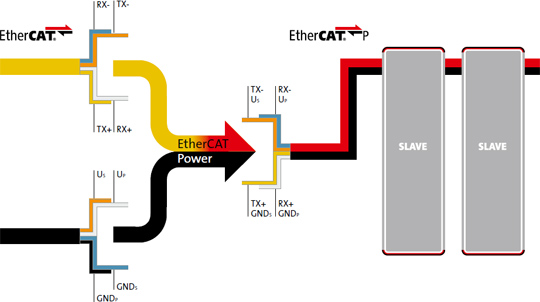
\includegraphics[width=\textwidth]{EtherCAT_Technology_04_EtherCATP.jpg}
	\caption{EtherCAT P example diagram \cite{protocol:ethercat}}
	\label{fig:ethercatp}
\end{figure}

Machines that include small parts with low power sensors and actuators can benefit from this addition by reducing the overall cabling complexity.
This creates cost-effective solutions with reduced wiring, possibly smaller form factor devices and lower system costs.
